\documentclass{beamer}

\usepackage{mpemath}
\usepackage{subcaption}
\usepackage[normalem]{ulem}
\usepackage{amsmath}
\usepackage{amssymb}
\usepackage{mathtools}
\usepackage{pgf}
\usepackage{pgfplots}
\usepackage{tikz}
\usepackage{booktabs}
\usepackage{siunitx}
\usepackage{natbib}
\usepackage{tabularx}
\usepackage{multirow}
\usepackage{amsmath}
\usepackage{mathtools}
\usepackage{amssymb}
\usepackage{bbm}
\usepackage[dvipsnames]{xcolor} % Saved my life during a conference once
\DeclareMathOperator{\regret}{Regret}
\DeclareMathOperator{\loss}{Loss}


\usetikzlibrary{arrows,automata,backgrounds,positioning,decorations,intersections,matrix}

% *** Styles ***
\usetheme{Singapore}
\setbeamertemplate{navigation symbols}{}
% \usetheme[progressbar=frametitle]{metropolis}
% \usecolortheme{dolphin}
%\useinnertheme{circles}
%\usecolortheme{rose}
%\setbeamercovered{transparent}
\setbeamercovered{invisible}
\usefonttheme{professionalfonts}
%\usefonttheme[onlymath]{serif}
\setbeamertemplate{footline}[frame number]

\title{ROIL -- Robust Offline Imitation Learning}
\author{Gersi Doko}
\institute{Department of Computer Science \\ University of New Hampshire}
\date{}

\AtBeginSection[]{
	\begin{frame}
          \vfill
	\centering
	% \usebeamerfont{title}
        {\huge\bf \insertsectionhead}%
	\vfill
\end{frame}
}

\begin{document}

\frame{\titlepage}

\section*{Intro}

\begin{frame}
	\frametitle{Imitation Learning}
	\centering
	\begin{minipage}{0.9\linewidth}
		\begin{figure}
			\centering
			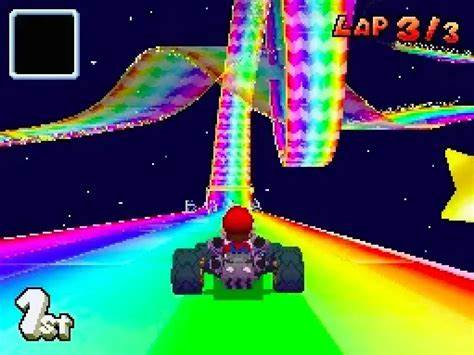
\includegraphics[width=\linewidth]{plots/rainbow_road.jpeg}
			% \caption{Super Mario Kart 64 Rainbow Road}
		\end{figure}
	\end{minipage}
\end{frame}

\begin{frame}
	\frametitle{Imitation Learning}
	\textbf{Objective}: Learn from expert demonstrations
	\begin{itemize}
		\item Health care: automating and improving ER care
		\item Robotics: self-driving cars, manufacturing, etc.
		\item Retail: recommendation systems, customer service
	\end{itemize}
	\vfill
	\textbf{Offline IL}: Given fixed dataset of expert demonstrations
	\begin{itemize}
		\item No interaction with the environment
	\end{itemize}
\end{frame}

\begin{frame}
\frametitle{Imitation Learning}
	\begin{itemize}
		\item RL requires rewards
		\vfill
		\item Rewards are hard to specify
		\vfill
		\item Often have access to expert demonstrations
		\vfill
		\item \emph{Key Idea}: Supervised learning from expert demonstrations
	\end{itemize}
\end{frame}

\begin{frame}
\frametitle{Imitation Learning}
	\textbf{Behavioral Cloning (BC)}: Supervised learning from expert demonstrations
	\[ 
		\min_{\theta} \sum_{(s,a)}^{D_e} \loss \left(\pi_\theta(s) - a \right)
	\]
	\vfill
	\textbf{Benefits}
	\begin{itemize}
		\item Simple, Natural, Easy to implement
	\end{itemize}
\end{frame}

\begin{frame}
	\frametitle{Imitation Learning Difficulties}
	\[ 
		\min_{\theta} \sum_{(s,a)}^{D_e} \loss \left(\pi_\theta(s) - a \right)
	\]
	\vfill
	\textbf{Central Issues}
	\begin{itemize}
		\item Sample inefficient
		\item Expert demonstrations may not be optimal
		\item Sensitive to dataset collection (e.g. an expert who only shows a subset of the state space)
	\end{itemize}
\end{frame}

\begin{frame}
	\frametitle{Inverse Reinforcement Learning}
	\textbf{Objective}: Learn from expert data
	\begin{itemize}
		\item Leverage model dynamics to reduce sample complexity
		\item Aims to match experts state-action distribution
		\item Known model dynamics allow for generalization
	\end{itemize}
	\vfill
	\textbf{Key Idea}: Learn a reward function from expert demonstrations, then use RL to learn a policy
\end{frame}

\begin{frame}
	\frametitle{Inverse Reinforcement Learning}
	\textbf{Objective}: Learn from expert data $D_e$
	\[ 
		\min_{\pi \in \Pi} \max_{r \in \mathcal{R}} \rho(\hat{\pi}_{D_e}, r) - \rho(\pi, r)
	\]
	\vfill
	\textbf{Benefits}
	\begin{itemize}
		\item Able to generalize to unseen states
		\item Can learn from suboptimal demonstrations
	\end{itemize}
	\vfill
	\textbf{Central Issues}
	\begin{itemize}
		\item \textcolor{blue}{Estimating the expert's policy $\hat{\pi}_{D_e}$}
	\end{itemize}
\end{frame}

\begin{frame}
\frametitle{Off-Policy IRL}
\begin{figure}
  \begin{center}
  \begin{minipage}{0.45\linewidth}
    \centering
    \emph{On-Policy}\\
    \textbf{True Expert $\pi_e$}
    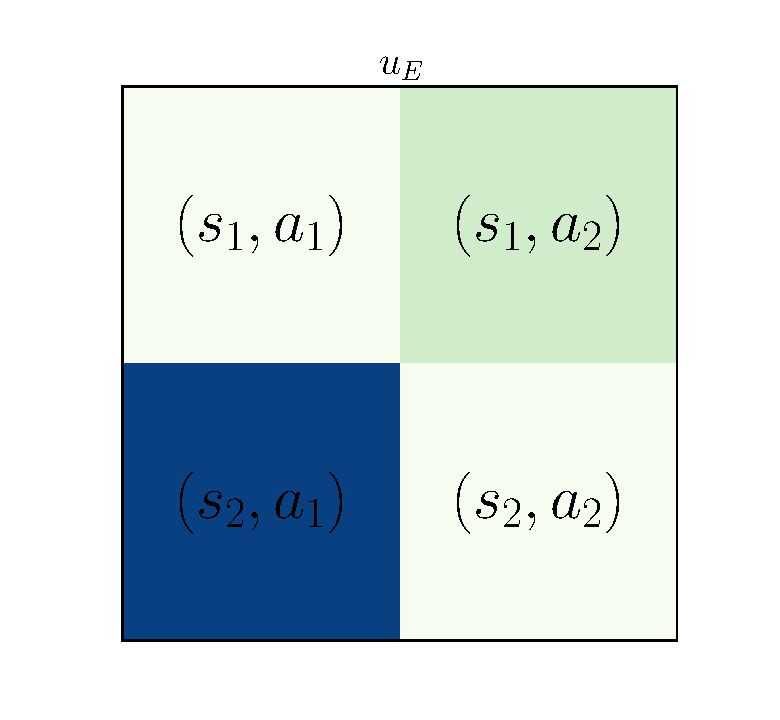
\includegraphics[width=\linewidth]{./plots/all_state/ue.pdf}
    LPAL Return $= 86/87$
  \end{minipage}
  \begin{minipage}{0.45\linewidth}
    \centering
    \emph{Off-Policy}\\
    \textbf{Estimated Expert $\hat{\pi}_{D_e}$}
    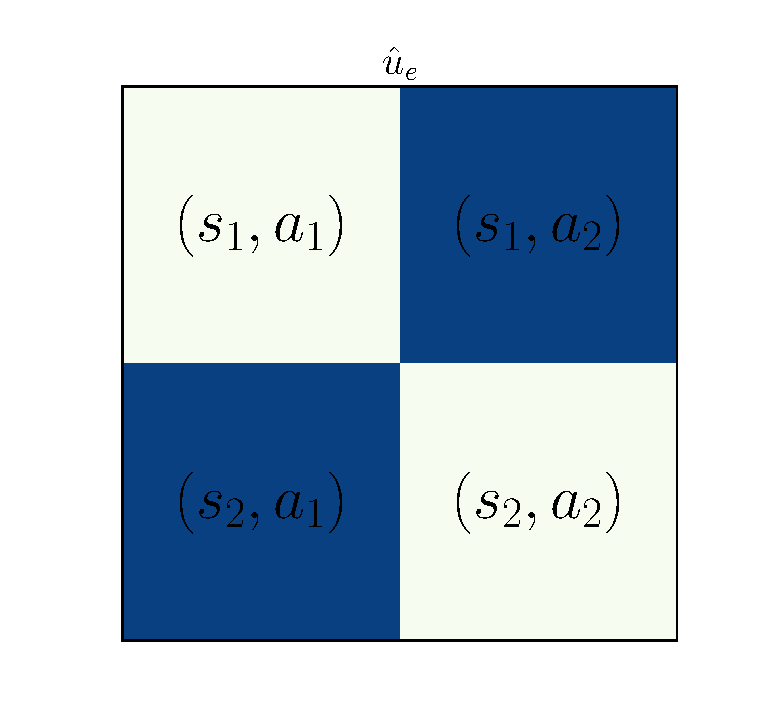
\includegraphics[width=\linewidth]{./plots/all_state/uehat.pdf}
    LPAL Return $= 38/87$
  \end{minipage}
  \end{center}
\end{figure}
\end{frame}

\begin{frame}
\frametitle{Off-Policy IRL}
\begin{figure}
  \begin{center}
  \begin{minipage}{0.45\linewidth}
    \centering
    \emph{On-Policy}\\
    \textbf{True Expert $\pi_e$}
    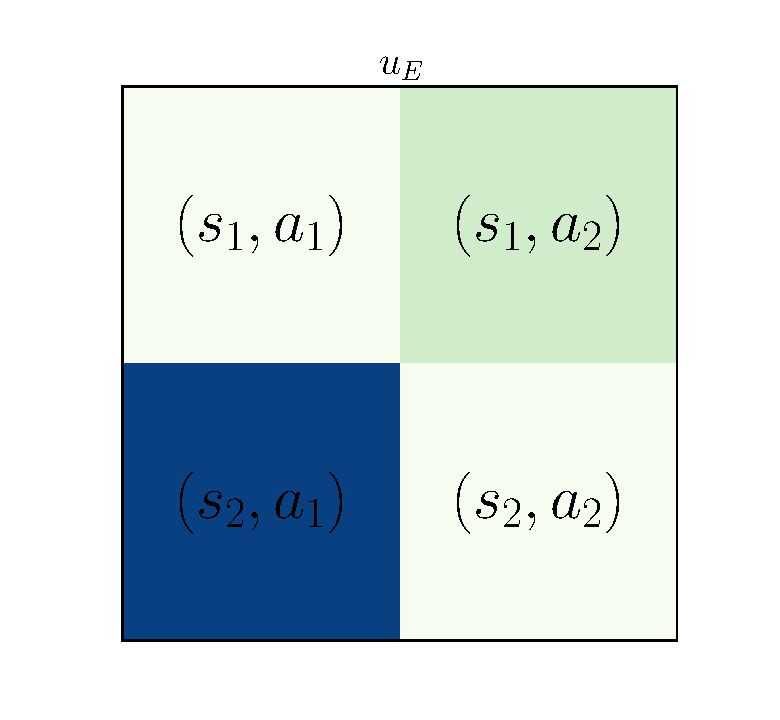
\includegraphics[width=\linewidth]{./plots/all_state/ue.pdf}
    LPAL Return $= 86/87$ \\
    \textcolor{green}{\textbf{ROIL Return $= 79/87$}}
  \end{minipage}
  \begin{minipage}{0.45\linewidth}
    \centering
    \emph{Off-Policy}\\
    \textbf{Estimated Expert $\hat{\pi}_{D_e}$}
    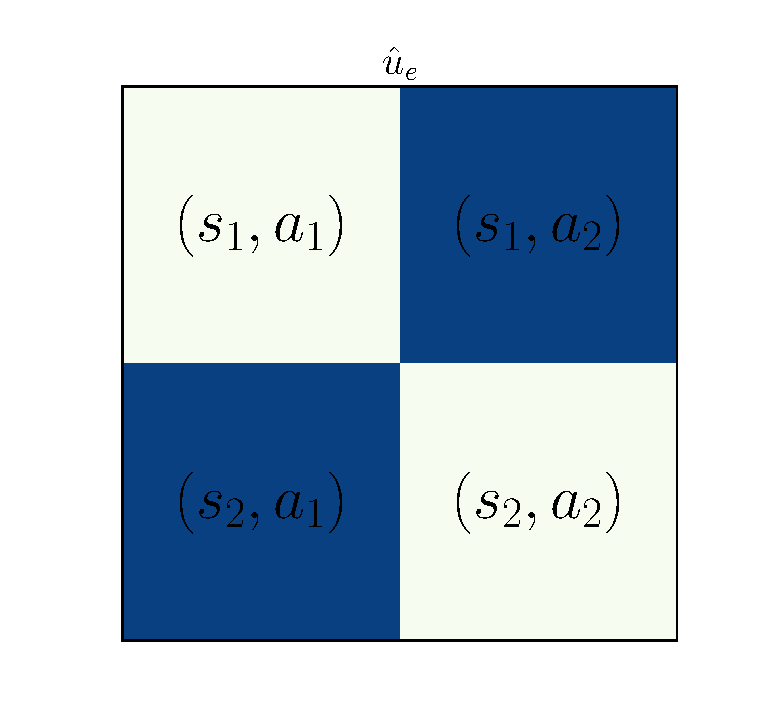
\includegraphics[width=\linewidth]{./plots/all_state/uehat.pdf}
    LPAL Return $= 38/87$ \\
    \textcolor{green}{\textbf{ROIL Return $= 82/87$}}
  \end{minipage}
  \end{center}
\end{figure}
\end{frame}

\begin{frame}
	\frametitle{This Talk}
	\textbf{Objective}: \textcolor{red}{Don't} estimate the expert's policy
	\[
		\min_{\pi \in \Pi} \max_{r \in \mathcal{R}} \rho(\textcolor{red}{\hat{\pi}_{D_e}}, r) - \rho(\pi, r)
	\]
	\vfill
	\textbf{Key Idea}: Minimize worst case regret
	\[
		\min_{\pi \in \Pi} \textcolor{blue}{\max_{\pi_e \in \Pi_{D_e}}} \max_{r \in \mathcal{R}} \rho(\textcolor{blue}{\pi_e}, r) - \rho(\pi, r)
	\]
\end{frame}

\section*{Preliminaries}

\begin{frame} \frametitle{Markov Decision Process}
  \textbf{Model} (tabular in this talk) \par
    {\small
   ~~~States $\mathcal{S}$: $s_1, s_2, s_3, \dots $ \par
   ~~~Actions $\mathcal{A}$: $a_1, a_2, \dots $ \par
   ~~~Transition probabilities $\mathcal{P} \in \Real^{\mathcal{S} \times \mathcal{A} \times \mathcal{S} }$ \par
   ~~~Initial state distribution $p_0 \in \Delta^\mathcal{S}$ \par
   ~~~Discount factor $\gamma \in \Real$ \par
   ~~~Features $\Phi \in \Real^{\mathcal{S} \mathcal{A} \times k}$ \par
   ~~~\sout{Rewards $r \in \Real^{\mathcal{S} \times \mathcal{A}}$}}
    \vfill 
    \textbf{Solution}: Policy ${\pi}\colon \mathcal{S} \to \Delta^\mathcal{A}$
    \vfill
    \textbf{Return}: Discounted expected infinite horizon return (expectation over trajectories):
    \[
	    \tilde{\rho}(\pi) = \lim_{T \to \infty} \sum_{t=0}^T \gamma^t r(\tilde{s}^{\pi}_t, \tilde{a}^{{\pi}}_t)
    \]
    \vfill
    \textbf{Random variables}: $\tilde{\rho}, \tilde{s}, \tilde{a}, \tilde{x}, \dots $ adorned with tilde
\end{frame}

% \begin{frame} \frametitle{Occupancy Frequencies}
% 	\[
% 		\mathcal{U}
% 		\; =\; 
% 		\left\{ u^{\pi} \mid  \pi \in \Pi \right\}
% 		\; =\;
% 		\Bigl\{ u\in \Real^{SA}_{+} \mid \sum_{a\in \mathcal{A}} (I - \gamma\cdot P\tr_a) \cdot u(\cdot, a) = p_0 \Bigr\}.
% 	\]
% 	Intuitively, $u_\pi(s,a)$ is the probability of agent $\pi$ being in state $s$ and taking action $a$.
% 	\[
% 		u_\pi(s,a) \propto \mathbb{P}(\tilde{s}_t = s, \tilde{a}_t = a \mid \tilde{s}_0 \sim p_0)
% 	\]
% \end{frame}
%
% \begin{frame} \frametitle{Consistent Occupancy Frequencies}
% 	We are given a dataset
% 	\[
% 		D_e = {(s_i, \pi_e(s_i))}_{i=1}^N.
% 	\]
% 	\textbf{Definition}: The set of consistent occupancy frequencies $\Upsilon$ is defined as
% 	\[
% 		\Upsilon = \left\{ u \in \mathcal{U} \mid u(s,a) = 0 \iff (s,a) \notin D_e \;\; \text{and} \;\; (s,a^\prime) \in D_e \right\},
% 	\]
% \end{frame}

% \begin{frame}
% 	\frametitle{Notation}
% 	\begin{itemize}
% 		\item Let $m, n$ be positive integers
% 		\item $\Real^{mn}$ denotes the set of $m \cdot n$-dimensional real vectors
% 		\item $\Real^{m \times n}$ denotes the set of $m \times n$ real matrices
% 		\item $\Delta^m$ denotes the $m$-dimensional probability simplex
% 		\item $\Pi$ denotes the set of all randomized Markov policies
% 	\end{itemize}
% \end{frame}

\begin{frame}
	\frametitle{Realizable Rewards}
	\textbf{Common assumption} : $r^\star$ can be realized by our features $\Phi \in \Real^{\mathcal{S}\mathcal{A} \times k}$
	and a weight vector $w \in \mathcal{W}$ such that $r^\star = \Phi w$.
	\vfill
	Prior work has restricted the weight vector to the L1 norm ball:
	\[ \mathcal{W} = \lbrace w \in \Real^k \mid \lvert \lvert w \rvert \rvert_1 \leq 1 \rbrace \]
	There are other viable choices of $\mathcal{W}$, which we accommodate for as an extension to our work.
\end{frame}

% \begin{frame}
% 	\frametitle{On-Policy vs Off-Policy}
% 	\begin{equation*} \label{eq:definition_u_hat}
% 	\hat{u}_e(s,a)
% 	\;=\; \sum_{(t, s',a') \in D_e} \gamma^t \cdot  \I{s=s' \wedge\; a=a'},
% 	\end{equation*}
% 	\vfill
% 	\begin{itemize}
% 		\item \textbf{Definition}: A set of demonstrations $D_e$ is said to be \emph{On Policy} if $$\lim_{N \to \infty} \| \hat{u}_e(D_e^N) - u_e \|_\infty  = 0$$
% 	\end{itemize}
% \end{frame}
% \section*{Our Approach}
%
% \begin{frame}
% 	\frametitle{Our Approach}
% 	\textbf{Problem}: Find a policy $\pi$ that minimizes the regret with respect to the worst case expert consistent with the demonstrations $D_e$.
% 	\[ \rho(\tilde{\pi}, r) = \lim_{t \to \infty} \mathbb{E}^{\tilde{\pi}, \mathcal{P}} \lbrack \sum_{t=0}^T \gamma^t r(\tilde{s_t}, \tilde{\pi}(\tilde{s_t})) \rbrack \]
% \end{frame}
%
% \begin{frame}
% 	\frametitle{Our Approach}
% 	\textbf{Problem}: Find a policy $\pi$ that minimizes the regret with respect to the worst case expert consistent with the demonstrations $D_e$.
% 	\[ \rho(\tilde{\pi}, r) = \lim_{t \to \infty} \mathbb{E}^{\tilde{\pi}, \mathcal{P}} \lbrack \sum_{t=0}^T \gamma^t r(\tilde{s_t}, \tilde{\pi}(\tilde{s_t})) \rbrack \]
% 	\[ \Pi_R(D) = \lbrace \pi \in \Pi \mid \pi(s,a) = 1 \quad \forall (s,a) \in D \rbrace \]
% \end{frame}

% \begin{frame}
% 	\frametitle{Our Approach}
% 	\textbf{Problem}: Find a policy $\pi$ that minimizes the regret with respect to the worst case expert consistent with the demonstrations $D_e$.
% 	\[ \rho(\tilde{\pi}, r) = \lim_{t \to \infty} \mathbb{E}^{\tilde{\pi}, \mathcal{P}} \lbrack \gamma^t r(\tilde{s_t}, \tilde{\pi}(\tilde{s_t})) \rbrack \]
% 	\[ \Pi_R(D) = \lbrace \pi \in \Pi \mid \pi(s,a) = 1 \quad \forall (s,a) \in D \rbrace \]
% 	\[ \min_{\pi \in \Pi_R(D_e)} \max_{\pi_e \in \Pi_R(D_e)} \max_{r \in \mathcal{R}} \rho(\pi_e, r) - \rho(\pi, r)\]
% \end{frame}

% \begin{frame}
% 	\frametitle{Our Approach}
% 	\[ \min_{\pi \in \Pi} \max_{\pi_e \in \Pi_R(D_e)} \max_{r \in \mathcal{R}} \rho(\pi_e, r) - \rho(\pi, r)\]
% 	\textbf{Observation}: The maximization over $\mathcal{R}$ may result in an intractable optimization problem.
% 	\textbf{Solution}: Recall the set of possible reward functions.
%         \[ \mathcal{W} = \lbrace w \in \Real^k \mid \lvert \lvert w \rvert \rvert_1 \leq 1 \rbrace \]
% 	\[ \mathcal{R} = \lbrace r \in \Real^{\mathcal{S} \mathcal{A}} \mid \exists w \in \mathcal{W}, \; r = \Phi w \rbrace \]
% 	\[ \min_{\pi \in \Pi_R(D_e)} \max_{\pi_e \in \Pi_R(D_e)} \max_{w \in \mathcal{W}} \rho(\pi_e, \Phi w) - \rho(\pi, \Phi w)\]
% \end{frame}

% \begin{frame}
% 	\frametitle{Our Approach}
% 	\textbf{Implementation Detail}: It can be difficult in practice to optimize over $\Pi$, and $\Pi_R(D_e)$ directly.\\
% 	\textbf{Solution}: Instead optimize over the occupancy frequencies of the policies.
% 	\[ \mathcal{U} = \lbrace u \in \RealPlus^{\mathcal{SA}} \mid \sum_{a \in \mathcal{A}} (I - \gamma \mathcal{P}_a\tr) \cdot u(\cdot, a) = p_0 \rbrace \]
% 	\[ \Upsilon = \lbrace u \in \mathcal{U} \mid u\tr c = 0 \rbrace \]
% 	\[ \text{where} \quad c(s,a) =
% 	\begin{cases}
% 	1 &\text{if  }
% 		(s,a) \notin \mathcal{D} \wedge
% 		\exists a'\in \mathcal{A}, (s, a') \in \mathcal{D}, \\
% 	0 & \text{otherwise}.
% 	\end{cases} \]
% 	\[ \min_{u \in \Upsilon} \max_{u_e \in \Upsilon} \max_{w \in \mathcal{W}} u_e\tr \Phi w - u\tr \Phi w\]
% \end{frame}

\section*{ROIL}
\begin{frame}
	\frametitle{ROIL: Robust Offline Imitation Learning}
	\[
		\min_{\pi \in \Pi} \textcolor{blue}{\max_{\pi_e \in \Pi_{D_e}}} \max_{r \in \mathcal{R}} \rho(\textcolor{blue}{\pi_e}, r) - \rho(\pi, r)
	\]
\end{frame}

\begin{frame}
	\frametitle{ROIL: Robust Offline Imitation Learning}
	\[ 
		\begin{mprog}
			\minimize{t \in \Real, u \in \Real^{\mathcal{S}\mathcal{A}}} t
			\stc t \geq \max_{u_e \in \Upsilon} u_e\tr r - u\tr r,\quad \forall \; r \in ext(\mathcal{R}),
			\cs u\in \Upsilon
		\end{mprog} 
	\]
\vfill

\begin{itemize}
	\item $ext(\mathcal{R})$ is the set of extreme points of $\mathcal{R}$
	\item $u$ is the occupancy frequency of our policy
	\item $t$ is the worst case regret
\end{itemize}
\end{frame}

\begin{frame}
	\frametitle{ROIL-P}
	\begin{itemize}
		\item \textbf{Key Strength}: ROIL does not estimate the expert's policy $\hat{\pi}_e$
		\vfill
		\item \textbf{Problem}: In on-policy domains, estimates of $\hat{\pi}_e$ are close to the true expert
		\vfill
		\item \textbf{Solution}: ROIL-P, a variant of ROIL that estimates $\hat{\pi}_e$, and prunes the set of reward functions
	\end{itemize}
\end{frame}

\begin{frame}
	\frametitle{ROIL-P}
	\textbf{Solution}: ROIL-P, a variant of ROIL that estimates the expert's occupancy frequency, and prunes the set of reward functions
	\vfill
	\[ 
	\begin{mprog}
		\minimize{t \in \Real, u \in \Real^{\mathcal{S} \times \mathcal{A}}} t
		\stc t \geq \max_{u_e \in \Upsilon} u_e\tr r - u\tr r,\quad \forall \; r \in ext(\textcolor{blue}{\lbrace r \in \mathcal{R} \mid \hat{u}_e\tr r >= 0 \rbrace}),
			\cs u\in \Upsilon
	\end{mprog} 
	\]
	% $\small{\Psi(\mathcal{R}) = \lbrace r \in \mathcal{R} \mid \hat{u}_e\tr r >= 0 \rbrace}$
\end{frame}

\section*{Example}

\begin{frame}
\frametitle{Example}

\begin{figure}
  \centering
	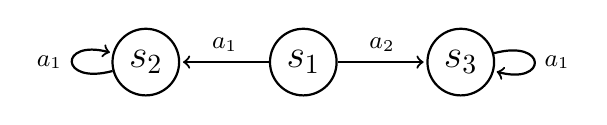
\begin{tikzpicture}[->,shorten >=1pt,auto,node distance=2cm,
		thick,main node/.style={circle,draw,font=\sffamily\Large\bfseries}]

	\node[main node] (1) {$s_1$};
	\node[main node] (2) [left of=1] {$s_2$};
	\node[main node] (3) [right of=1] {$s_3$};

	\path[every node/.style={font=\sffamily\small}]
	(1) edge node [above] {$a_1$} (2)
	edge node [above] {$a_2$} (3)
	(2) edge [loop left] node {$a_1$} (2)
	(3) edge [loop right] node {$a_1$} (3);
	\end{tikzpicture}
\end{figure}
\end{frame}

\begin{frame}

\begin{figure}
  \centering
  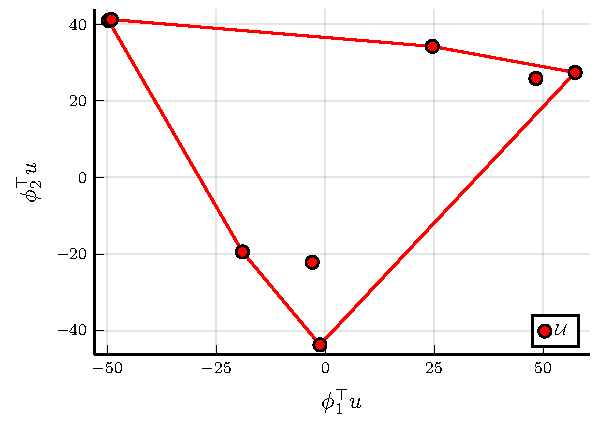
\includegraphics[width=\linewidth]{plots/visual_U.pdf}
\end{figure}
\end{frame}

\begin{frame}

\begin{figure}
  \centering
  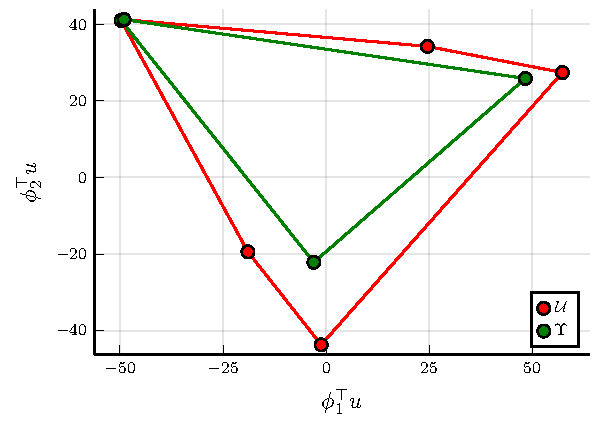
\includegraphics[width=\linewidth]{plots/visual_U_and_Upsilon.pdf}
\end{figure}
\end{frame}

\begin{frame}

\begin{figure}
  \centering
  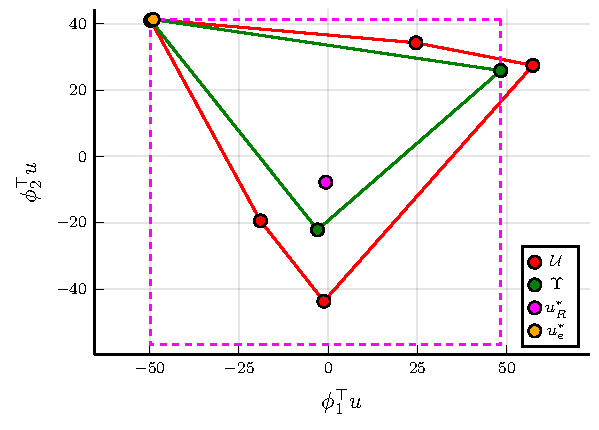
\includegraphics[width=\linewidth]{plots/visual_solve_cheb.pdf}
\end{figure}
\end{frame}

\begin{frame}
\frametitle{A Surprising Failure}
\begin{figure}
  \centering
	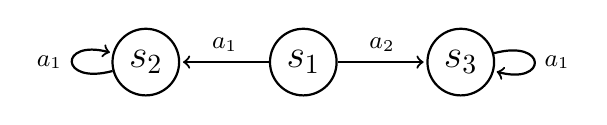
\begin{tikzpicture}[->,shorten >=1pt,auto,node distance=2cm,thick,main node/.style={circle,draw,font=\sffamily\Large\bfseries}]

	\node[main node] (1) {$s_1$};
	\node[main node] (2) [left of=1] {$s_2$};
	\node[main node] (3) [right of=1] {$s_3$};

	\path[every node/.style={font=\sffamily\small}]
	(1) edge node [above] {$a_1$} (2)
	edge node [above] {$a_2$} (3)
	(2) edge [loop left] node {$a_1$} (2)
	(3) edge [loop right] node {$a_1$} (3);
	\end{tikzpicture}
\end{figure}
\vfill
\[
	D_e = \lbrace (s_1, a_1), (s_2, a_1), (s_3, a_1) \rbrace
\]
\end{frame}

\begin{frame}
\frametitle{A Surprising Failure}
\begin{figure}
  \centering
	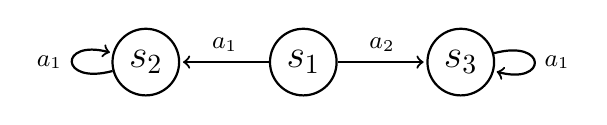
\begin{tikzpicture}[->,shorten >=1pt,auto,node distance=2cm,thick,main node/.style={circle,draw,font=\sffamily\Large\bfseries}]

	\node[main node] (1) {$s_1$};
	\node[main node] (2) [left of=1] {$s_2$};
	\node[main node] (3) [right of=1] {$s_3$};

	\path[every node/.style={font=\sffamily\small}]
	(1) edge node [above] {$a_1$} (2)
	edge node [above] {$a_2$} (3)
	(2) edge [loop left] node {$a_1$} (2)
	(3) edge [loop right] node {$a_1$} (3);
	\end{tikzpicture}
\end{figure}
\vfill
\[
	D_e = \lbrace (s_1, a_1), (s_2, a_1), (s_3, a_1) \rbrace
\]
\vfill
\begin{center}
	\textcolor{green}{ROIL Return $= 100\%$}\\
	\textcolor{red}{LPAL Return $= 50\%$}\\
	\textcolor{red}{GAIL Return $= 50\%$}\\
\end{center}

\end{frame}

\begin{frame}
\frametitle{A Surprising Failure}
\begin{figure}
  \begin{center}
  \begin{minipage}{0.46\linewidth}
    \centering
    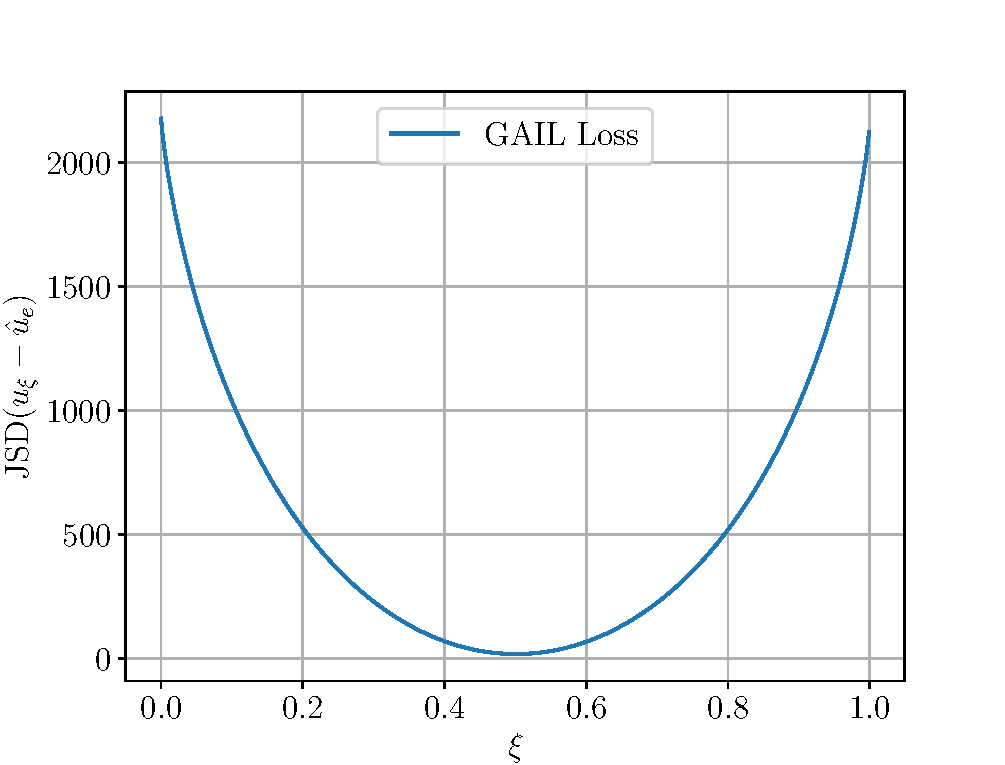
\includegraphics[width=\linewidth]{plots/all_state/gail_loss.pdf}
    \subcaption{On-Policy}
  \end{minipage}
  \hspace{0.05\linewidth}
  \begin{minipage}{0.46\linewidth}
    \centering
    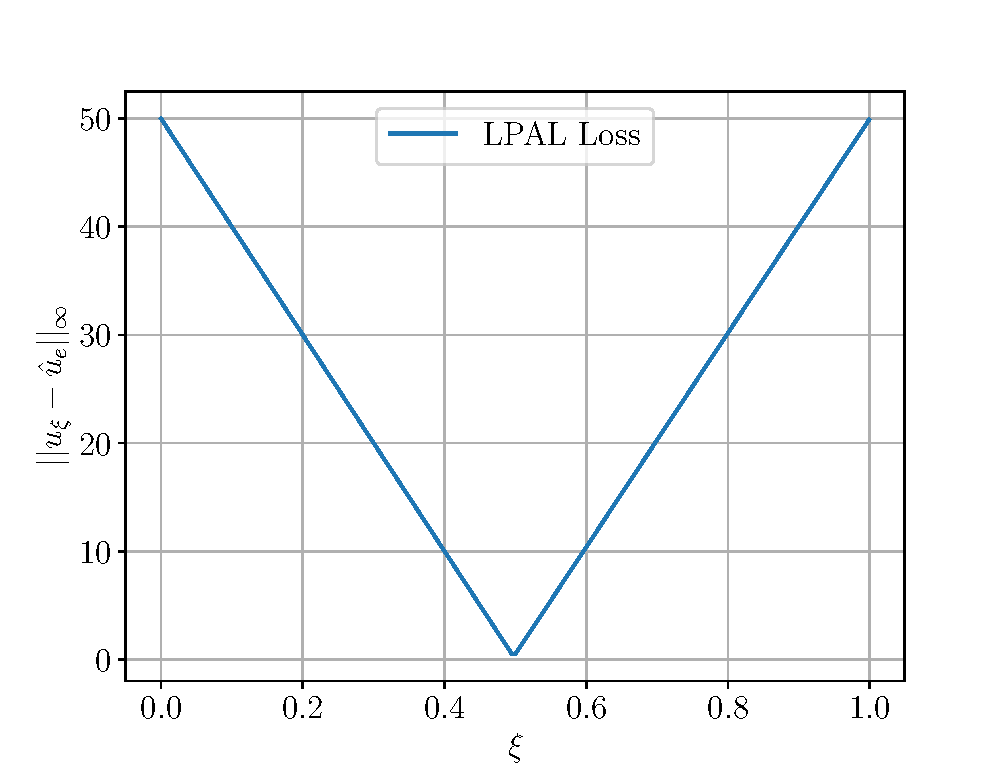
\includegraphics[width=\linewidth]{plots/all_state/lpal_loss.pdf}
    \subcaption{Off-Policy}
  \end{minipage}
  \end{center}
\end{figure}
\end{frame}

\section*{Experiments}

\begin{frame}
\frametitle{40x40 Gridworld}

\begin{figure}
  \begin{center}
  \begin{minipage}{0.46\linewidth}
    \centering
    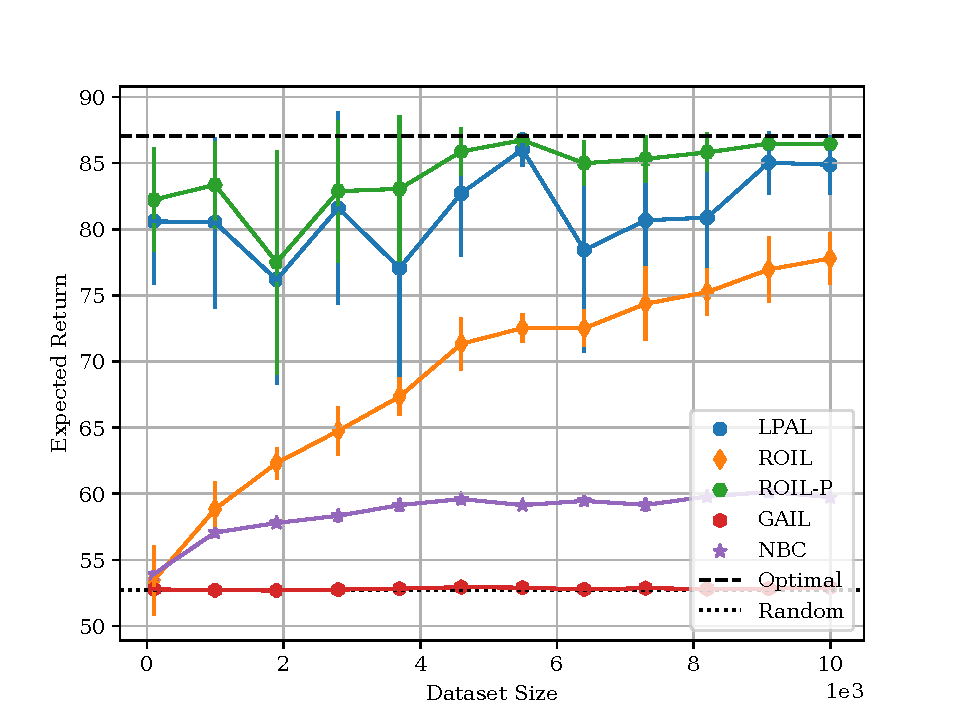
\includegraphics[width=\linewidth]{plots/returns/40x40_gridworld_on_policy_returns.pdf}
    \subcaption{On-Policy}
  \end{minipage}
  \hspace{0.05\linewidth}
  \begin{minipage}{0.46\linewidth}
    \centering
    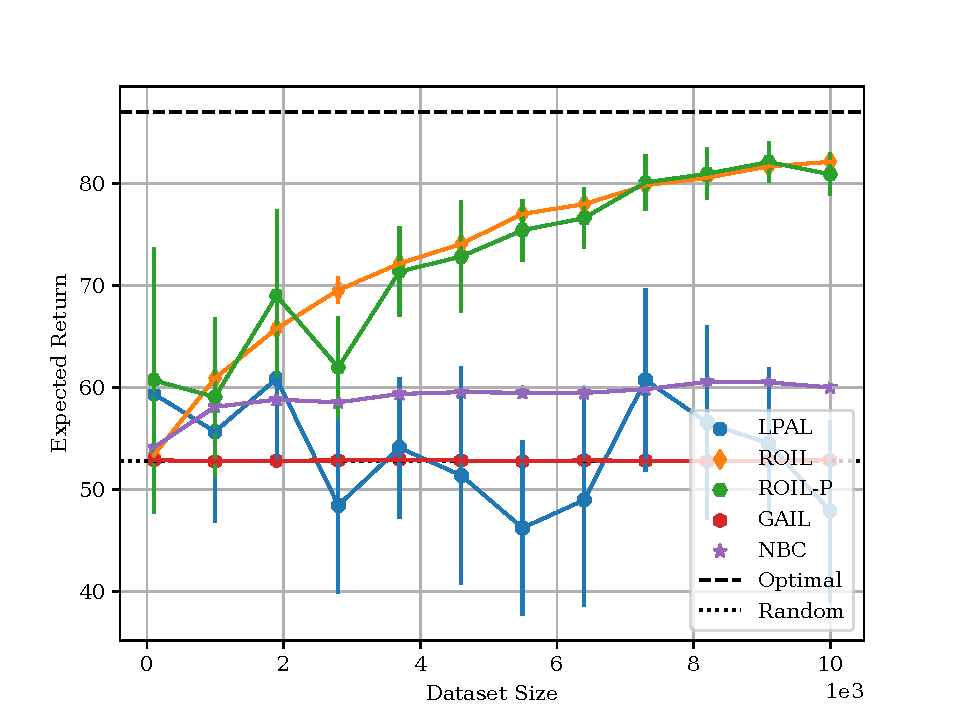
\includegraphics[width=\linewidth]{plots/returns/40x40_gridworld_off_policy_returns.pdf}
    \subcaption{Off-Policy}
  \end{minipage}
  \end{center}
\end{figure}

\end{frame}

\begin{frame}
	\frametitle{40x40 Driving Simulator}
\begin{figure}
  \begin{center}
  \begin{minipage}{0.46\linewidth}
    \centering
    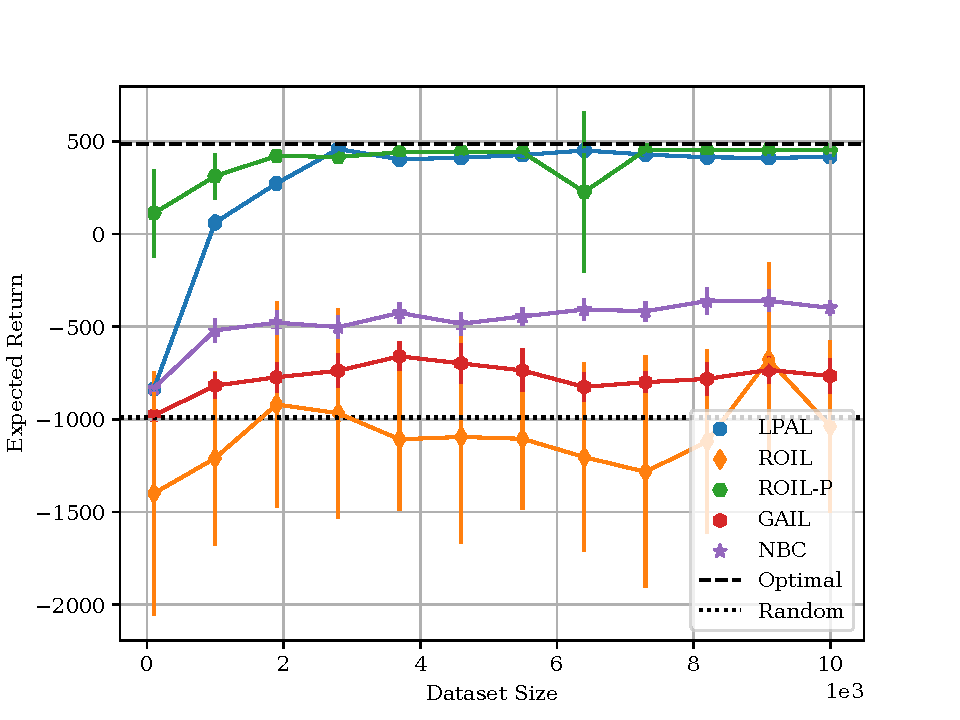
\includegraphics[width=\linewidth]{plots/returns/40x40_driving_on_policy_returns.pdf}
    \subcaption{On-Policy}
  \end{minipage}
  \hspace{0.05\linewidth}
  \begin{minipage}{0.46\linewidth}
    \centering
    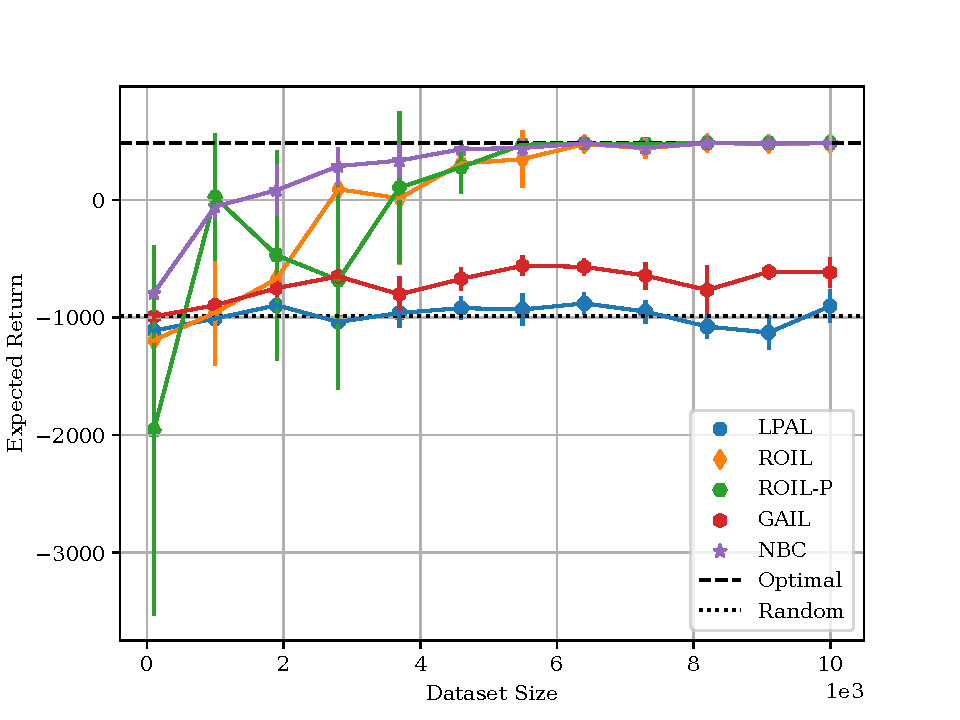
\includegraphics[width=\linewidth]{plots/returns/40x40_driving_off_policy_returns.pdf}
    \subcaption{Off-Policy}
  \end{minipage}
  \end{center}
\end{figure}
\end{frame}

\begin{frame}
\frametitle{Regret Comparison}

\[ \regret(\pi) = \max_{\pi_e \in \Pi_{D_e}} \max_{r \in \mathcal{R}} \rho(\pi_e, r) - \rho(\pi, r)\]

\begin{figure}
  \begin{center}
  \begin{minipage}{0.46\linewidth}
    \centering
    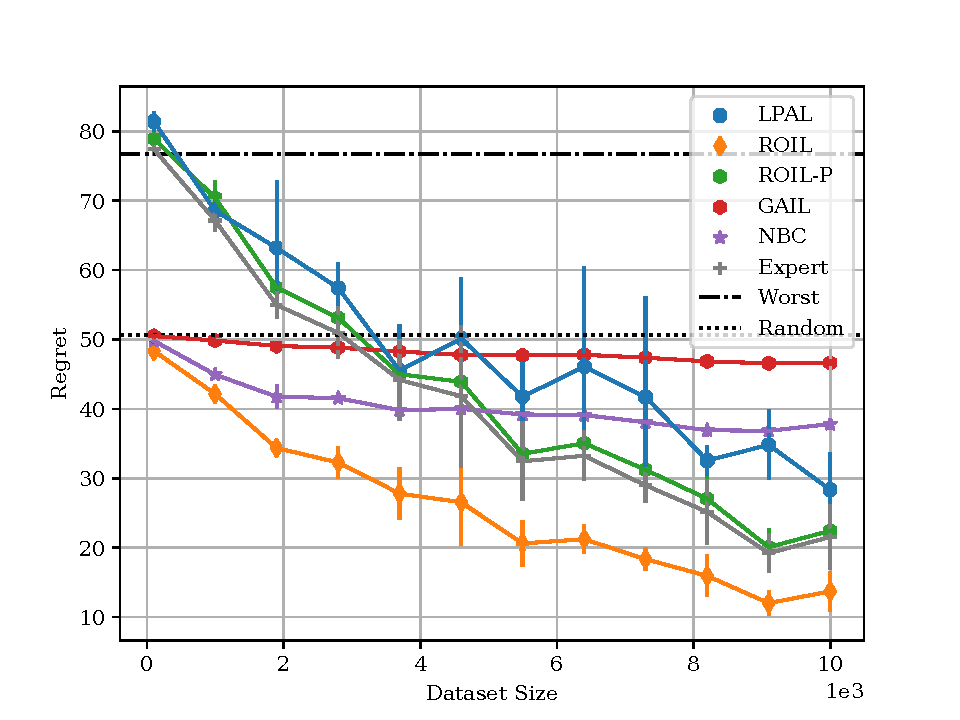
\includegraphics[width=\linewidth]{plots/regrets/40x40_gridworld_on_policy_regret_regrets.pdf}
    \subcaption{On-Policy}
  \end{minipage}
  \hspace{0.05\linewidth}
  \begin{minipage}{0.46\linewidth}
    \centering
    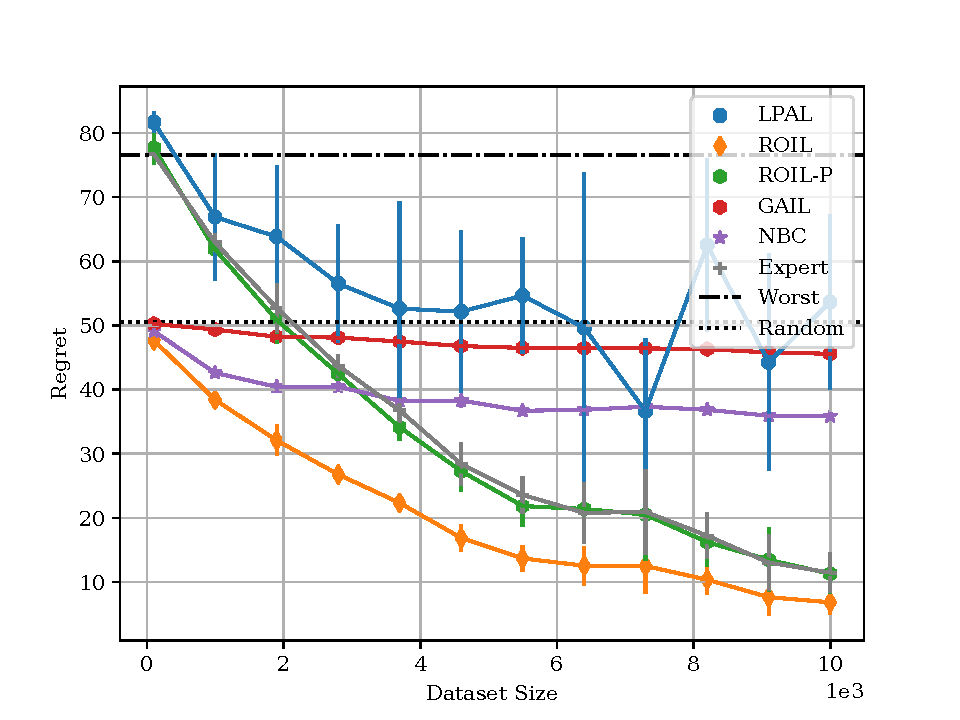
\includegraphics[width=\linewidth]{plots/regrets/40x40_gridworld_off_policy_regret_regrets.pdf}
    \subcaption{Off-Policy}
  \end{minipage}
  \end{center}
\end{figure}
\end{frame}

\begin{frame}
	\frametitle{Conclusion}
	\begin{itemize}
		\item Need offline IRL methods that are robust to covariate shift
		\vfill
		\item Existing methods fail to learn a robust policy
		\vfill
		\item ROIL is a principled approach to solving the robust offline IRL problem
	\end{itemize}
\end{frame}

\end{document} 
